\documentclass{article}
\usepackage[polish]{babel}
\usepackage[utf8]{inputenc}
\usepackage[T1]{fontenc}
\usepackage{graphicx}
\usepackage{amsmath}
\usepackage{listings}
\usepackage{lmodern}
\usepackage[margin=0.75in]{geometry}
\usepackage{float}
\usepackage[export]{adjustbox}
\usepackage{xcolor}
\usepackage{sectsty}
\usepackage{titlesec}
\usepackage{indentfirst}
\titlelabel{\thetitle.\quad}
\definecolor{Myblue}{rgb}{0.14,0.4,0.74}
\definecolor{Myblue2}{rgb}{0.14,0.6,0.84}
\sectionfont{\color{Myblue}}
\subsectionfont{\color{Myblue2}}
\definecolor{codepurple}{HTML}{C42043}

\begin{document}
\begin{titlepage}
   \vspace*{80mm}
   \centering
   \noindent\makebox[\linewidth]{\rule{\paperwidth}{0.4pt}}
   \LARGE{\textsc{Aplikacja giełdowa}\\}
   Platformy programistyczne .Net i Java\\
   \textsc{\large mgr inż. Aneta Górniak\\}
   \large \today \\
   \noindent\makebox[\linewidth]{\rule{\paperwidth}{0.4pt}}
   \begin{minipage}[l]{0.3\textwidth}
      \vspace{0.4cm}
      Autorzy:\\
      \textsc{\large Emilia Starczyk} 249005\\
      \textsc{\large Michał Kaleta} 248976\\
   \end{minipage}

   \vfill
\end{titlepage}
\section{Przeznaczenie aplikacji}
Aplikacja ``Finance Tracker'' pozwala na śledzenie przebiegu cen akcji na rynku
oraz sprawdzenia jej aktualnej ceny. Możliwe jest również symulowanie kupna
zadanej ilości akcji i dodania ich do wirtualnego portfela, w celu późniejszej
symulacji sprzedaży z zyskiem lub stratą.
\section{Funkcjonalność aplikacji}
\begin{figure*}[h]
    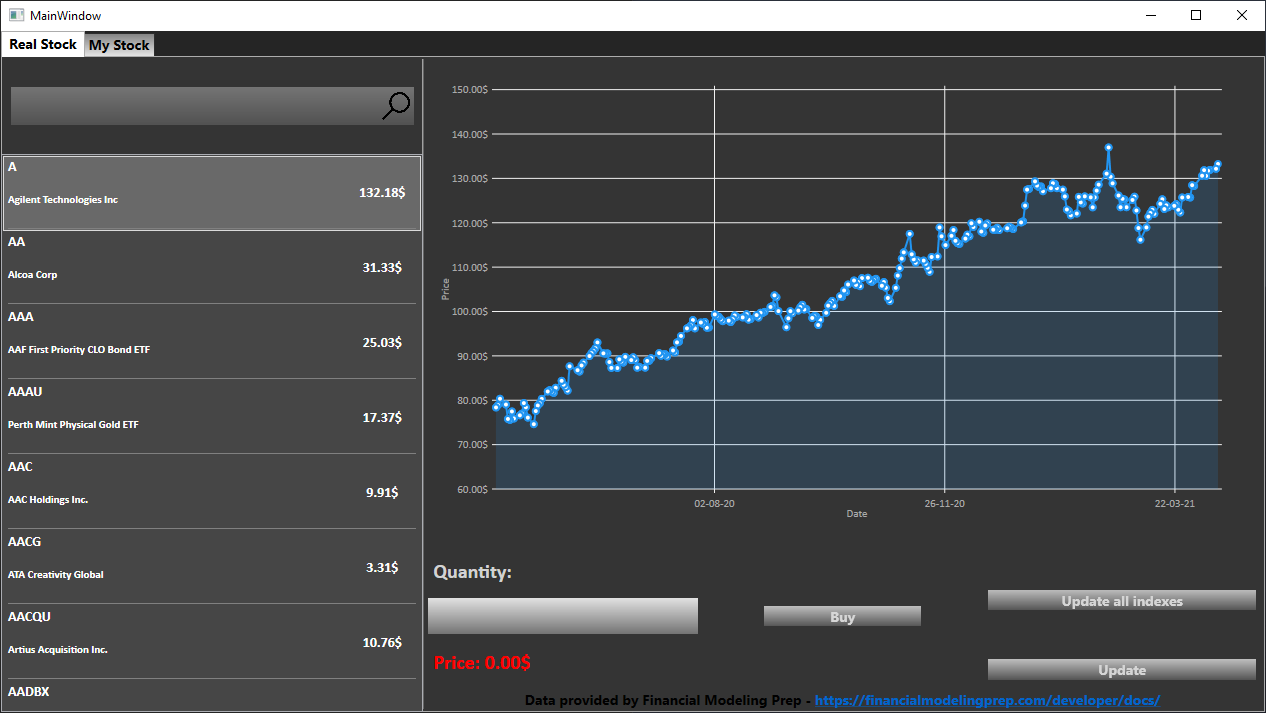
\includegraphics[width=\textwidth]{Ekran1.png}
    \caption{Ekran główny}
\end{figure*}
\large{
Główny ekran przedstawia listę dostępnych akcji na rynku. Lista po lewej stronie
jest przewijalna i przedstawia symbol akcji na giełdzie, pełną nazwę spółki oraz
jej aktualną cenę. Pole wyszukiwania w górnej części pozwala na filtrowanie indeksów
zawierających wpisane litery w symbolu.

Prawa strona przedstawia wykres ceny w czasie dla aktualnie wybranego indeksu. W
dolnej części użytkownik może symulować zakup wybranej ilości akcji danej
spółki. Po wpisaniu ilości w pole \textbf{Quantity} cena poniżej zaktualizuje się do
wartości jaką należałoby zapłacić za taką ilość akcji. Poprawność wpisanego
tekstu do pola \textbf{Quantity} jest sprawdzana wyrażeniem regularnym pozwalającym na
wpisanie jedynie liczb nie zaczynających się od 0. Kliknięcie przycisku \textbf{Buy}
dodaje wybraną ilość akcji do wirtualnego portfela dostępnego w drugiej
zakładce.

Przycisk \textbf{Update all indexes} służy do pobrania danych o aktualnych
cenach wszystkich indeksów dostępnych na giełdzie z zewnętrznego serwera.

Przycisk \textbf{Update} służy do pobrania danych o cenach historycznych
wybranego indeksu z zewnętrznego serwera.

Manualne pobieranie danych z serwera zewnętrznego zostało podyktowane
ograniczeniem dziennej ilości zapytań do 250.
}

\newpage
\begin{figure*}[ht]
    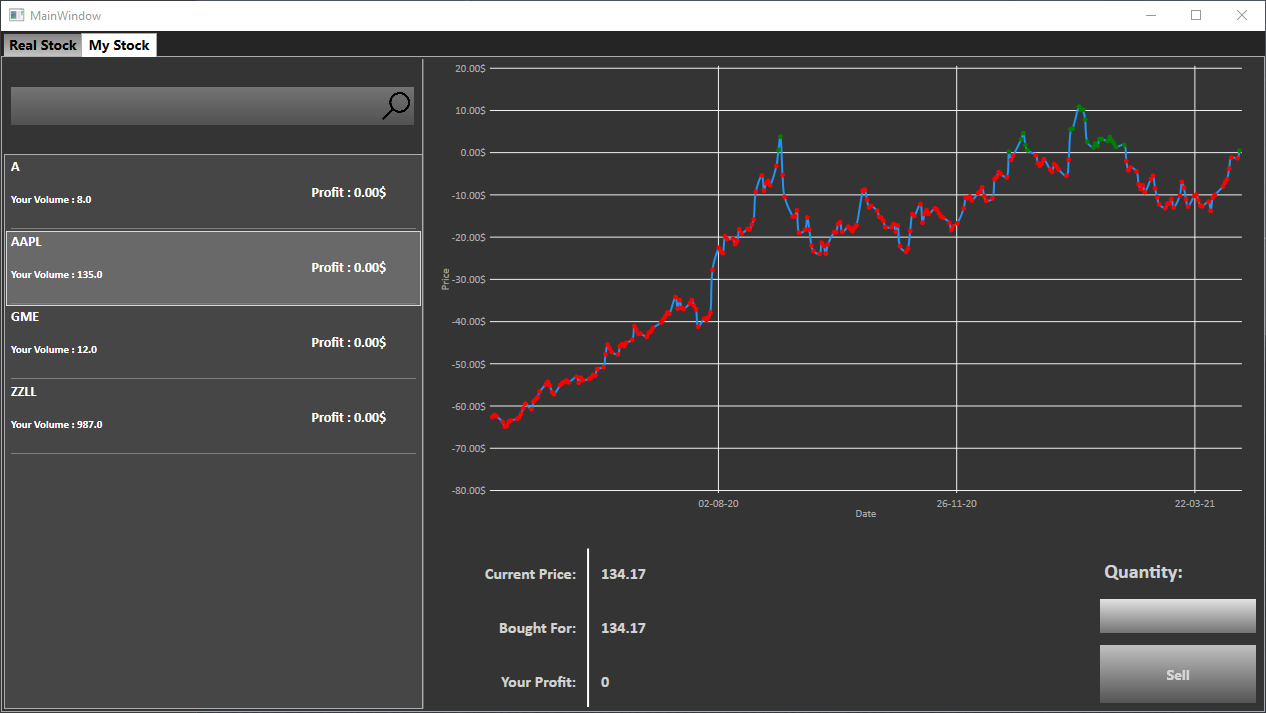
\includegraphics[width=\textwidth]{Ekran2.png}
    \caption{Ekran portfela użytkownika}
\end{figure*}
\large{
Ekran portfela użytkownika przedstawia wszystkie aktualnie posiadane akcje.
Znajdują się one na liście po lewej stronie. Wyświetlane są tam infromacje, o tym
jaka akcja znajduje się w portfelu, ile akcji zostało zakupionych oraz jaki jest
aktualny zarobek lub strata. Zakupienie tej samej akcji dwukrotnie jest liczone
jako osobna transakcja i tak też będzie wyświetlana w portfelu. Pole
wyszukiwania w górnej części pozwala na filtrowanie zakupionych akcji według
liter w symbolu.

Po prawej stronie znajduje się wykres zarobków w czasie. Czerwone punkty
symbolizują stratę, a zielone zysk. Poniżej wykresu wyświetlone są informacje na
temat aktualnej ceny akcji, ceny za jaką kupiliśmy dane akcje oraz aktualny zysk
lub strata.

Po prawej stronie znajduje się pole do wpisania ilości akcji, które chcemy
sprzedać. Pole to podlega takim samym restykcjom wpisywania, jak przy zakupie -
możliwe do wpisania są tylko liczby nie rozpoczynające się od 0. Po kliknięciu
przycisku \textbf{Sell} pojawi się okno pytające, czy napewno chcemy sprzedać
\textbf{n} akcji firmy \textbf{x} z zyskiem \textbf{y}. Jeśli wpisana przez nas
ilość przekracza posiadą ilość wybranej akcji, pojawi się okno informujące o tym
użytkownika.
}
    \begin{figure*}[h]
        \centering
        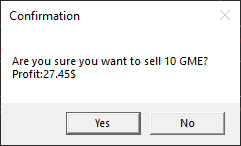
\includegraphics{sell.png}
        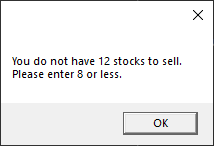
\includegraphics{brak.png}
    \end{figure*}  
\end{document}